% Generated by experiments/fig_reference.py from paper/reference.py; do not edit.
\begin{landscape}
\section{A serial reference implementation}
\label{app:reference}

\noindent\begin{minipage}[t]{0.405\linewidth}\vspace{0pt}\raggedright
{\small This is the complete algorithm: the file \texttt{shufflesnap/reference.py} from the
package, split into its parts, each beside a diagram computed with its code. Without exact
ties it returns the same assignment as the compiled kernel; the package's tests check this
for every preset on six kinds of target, from an exact-fit square to surplus cells and a
random mask. The kernel adds threads, skips windows whose cells have not changed (which does
not change the result) and an optional time budget. Points are in grid units: cell $(x,y)$
has its center at $(x,y)$.\par}
\end{minipage}\hfill
\begin{minipage}[t]{0.565\linewidth}\vspace{0pt}
\lstinputlisting[firstline=1,lastline=12,firstnumber=1,numbers=left,numberstyle=\tiny\color{black!45},numbersep=6pt,frame=none,xleftmargin=1.6em,aboveskip=0pt,belowskip=0pt]{reference.py}
\end{minipage}

\vspace{1.4em}
\noindent\begin{minipage}[t]{0.405\linewidth}\vspace{0pt}\raggedright
\textbf{The schedule.}\par\smallskip
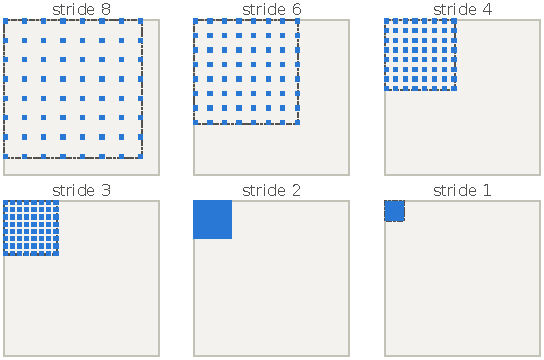
\includegraphics[width=\linewidth]{figures/fig_ref_schedule}\par\smallskip
{\small A window always holds $w\times w$ cells, but at stride $s$ they lie $s$ cells apart, so
it spans $(w-1)s+1$ cells per axis (dashed). The first stride is the smallest power of two
with $ws\ge L$, so the first windows reach across the axis; each later stride is the last one
divided by \texttt{ratio} and rounded. Each axis has its own strides, and the shorter axis
waits at 1. Drawn: one window of the default preset ($w=8$) on a $64\times64$ grid at every
stride.\par}
\end{minipage}\hfill
\begin{minipage}[t]{0.565\linewidth}\vspace{0pt}
\lstinputlisting[firstline=15,lastline=34,firstnumber=15,numbers=left,numberstyle=\tiny\color{black!45},numbersep=6pt,frame=none,xleftmargin=1.6em,aboveskip=0pt,belowskip=0pt]{reference.py}
\end{minipage}

\clearpage
\noindent\begin{minipage}[t]{0.405\linewidth}\vspace{0pt}\raggedright
\textbf{The windows of one tiling.}\par\smallskip
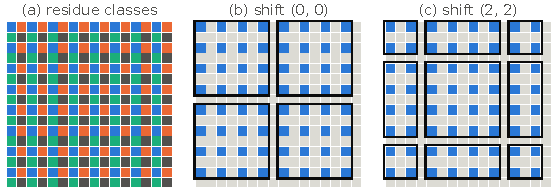
\includegraphics[width=\linewidth]{figures/fig_ref_windows}\par\smallskip
{\small At stride $(s_x,s_y)$ the cells fall into $s_xs_y$ residue classes $(x \bmod s_x,\,
y \bmod s_y)$ (a). In its class, cell $x$ is lattice column $x /\!/ s_x$, and tiles of $w$
lattice columns start at column \texttt{ox}. A window is the set of cells that share a class
and a tile (b, boxes). The four tilings of a round shift the tiles by half a window (c). Edge
windows are smaller, and masked cells never appear. Drawn with $w=4$, stride 2, class
$(0,0)$.\par}
\end{minipage}\hfill
\begin{minipage}[t]{0.565\linewidth}\vspace{0pt}
\lstinputlisting[firstline=37,lastline=44,firstnumber=37,numbers=left,numberstyle=\tiny\color{black!45},numbersep=6pt,frame=none,xleftmargin=1.6em,aboveskip=0pt,belowskip=0pt]{reference.py}
\end{minipage}

\vspace{1.4em}
\noindent\begin{minipage}[t]{0.405\linewidth}\vspace{0pt}\raggedright
\textbf{One window.}\par\smallskip
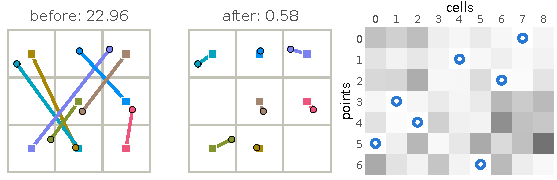
\includegraphics[width=\linewidth]{figures/fig_ref_solve}\par\smallskip
{\small The window's points are reassigned among all of its cells, empty ones included, by an
exact linear assignment on squared distances. The result is kept only if it lowers the
window's cost by more than a relative \texttt{tol}, so the cost never rises and ties cannot
cycle. \texttt{pos} gives each point's cell and \texttt{occ} each cell's point. Drawn: seven
points in a $3\times3$ window before and after, with summed squared distances, and the cost
matrix with the chosen entries.\par}
\end{minipage}\hfill
\begin{minipage}[t]{0.565\linewidth}\vspace{0pt}
\lstinputlisting[firstline=47,lastline=59,firstnumber=47,numbers=left,numberstyle=\tiny\color{black!45},numbersep=6pt,frame=none,xleftmargin=1.6em,aboveskip=0pt,belowskip=0pt]{reference.py}
\end{minipage}

\clearpage
\noindent\begin{minipage}[t]{0.405\linewidth}\vspace{0pt}\raggedright
\textbf{The whole method.}\par\smallskip
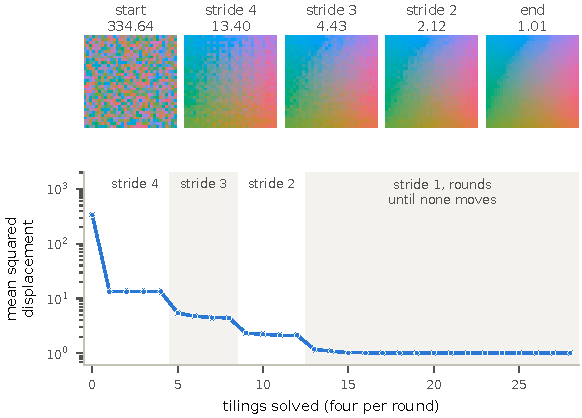
\includegraphics[width=\linewidth]{figures/fig_ref_snap}\par\smallskip
{\small The cells are the mask's usable entries in row-major order, and point $i$ starts in a
random cell \texttt{pos[i]}. A round solves the windows of the four tilings in turn. Each
coarse stage runs one round; then stride-1 rounds repeat until one moves nothing, a fixed
point of every window but not a proof of optimality. Drawn: 1{,}024 uniform points on a
$32\times32$ grid, colored by input position, after the start, each
coarse stage and the end (top), and the mean squared displacement in cells$^2$ after every
tiling (bottom): each stride halves it or better, and the last stride-1 round moves
nothing.\par}
\end{minipage}\hfill
\begin{minipage}[t]{0.565\linewidth}\vspace{0pt}
\lstinputlisting[firstline=62,lastline=83,firstnumber=62,numbers=left,numberstyle=\tiny\color{black!45},numbersep=6pt,frame=none,xleftmargin=1.6em,aboveskip=0pt,belowskip=0pt]{reference.py}
\end{minipage}
\end{landscape}
